% ISEG MASTER DISSERTATION TEMPLATE
% MASTER'S IN_____________
% AUTHOR:_________________
% SUPERVISER:___________________
%
% DISCLAIMER: This template is intended to help ISEG master's students producing their master's dissertation. It follows the guidelines set by Costa (2017). Note that for convenience this template does not use a bibliographic manager (e.g. JabRef), although it is highly recommendable (more on this on the 'References' below). I thank Professor Paulo Brito for helpful comments.
%
% Domingos Guerreiro Seward 25.06.2018
%
%
%  === PREAMBLE ============
%
% Define the document class 'book'.
% Set font size to 12, set to  A4 paper, and one-sided document.
\documentclass [12pt,a4paper,oneside]{article}

% Set font type to 'Times New Roman'.
\usepackage{times}

% Portuguese accents just in case.
\usepackage[T1]{fontenc}
\usepackage[utf8]{inputenc}

% English language.
\usepackage[english]{babel}

% appendix 
\usepackage[titletoc,toc,title]{appendix}
\newcommand{\nocontentsline}[3]{}
\newcommand{\tocless}[2]{\bgroup\let\addcontentsline=\nocontentsline#1{#2}\egroup}

\makeatletter

\def\@biblabel#1{\hspace*{-\labelsep}}

\makeatother

% Set margins to 3cm.
\usepackage[top=3cm, bottom=3cm, left=3cm, right=3cm]{geometry}

% Change margins command.
\def\changemargin#1#2{\list{}{\rightmargin#2\leftmargin#1}\item[]}
\let\endchangemargin=\endlist 

% Paragraph indentation.
\usepackage{indentfirst}

% Set vertical spacing to 1.5 lines.
\usepackage{setspace}
\onehalfspacing

% Page headers and footers customisation.
\usepackage{fancyhdr}
\pagestyle{fancy}
\fancyhf{}
	% Set left header to footnotesize (10pt) and upper cases.
\lhead{\footnotesize \textsc{Luís F. Costa}}
	% Set left header to footnotesize (10pt) and upper cases.
\rhead{\footnotesize\textsc{Template for MFW at ISEG}}
	% Set centred footer to page number.
\cfoot{\thepage}


% Customise chapters, sections, subsections, and subsubsections.
\usepackage{titlesec}
	% Set chapters' titles to upper cases and centred.
\titleformat{\chapter}[display]
  {\scshape\center}
  {}
  {0pt}
  {\thechapter.\ }
  \usepackage{etoolbox}% Stop chapters from starting at new page.
\makeatletter
\patchcmd{\chapter}{\if@openright\cleardoublepage\else\clearpage\fi}{}{}{}
\makeatother
	% Set sections' titles to upper cases and centred.
\titleformat{\section}
  {\scshape\center}{\thesection}{1em}{}
	% Set subsections' titles to italic and centred.
\titleformat{\subsection}
  {\itshape\center}{\thesubsection}{1em}{}
	% Idem for subsubsections' titles.
\titleformat{\subsubsection}
  {\itshape\center}{\thesubsection}{1em}{}


% Link objects (e.g. tables, figures, pages) in the body of text.
\usepackage{hyperref}

% Build a glossary.
\usepackage{glossaries}
\makeglossaries  
  % Define, e.g. acronyms (\newacronym{<label>}{<abbrv>}{<full>}).
  % Use \gls{<label>} command to call the acronym in the text. On first use the \gls command will display "<full> (<abbrv>)". On subsequent uses only the abbreviation will be displayed.

  \newacronym{gdp}{GDP}{Gross Domestic Product}
  \newacronym{jel}{JEL}{Journal of Economic Literature}
  \newacronym{mfw}{MFW}{Master's Final Work}
  \newacronym{ols}{OLS}{Ordinary Least Squares}

% Customize table of contents.
\usepackage{tocloft}
\setlength{\cftbeforetoctitleskip}{0pt}
%	\addto\captionsenglish{%
%	\renewcommand{\contentsname}{\hfill\normalfont\scshape\normalsize Table of Contents\hfill}   
	%\renewcommand{\cftaftertoctitle}{\hfill}
%	}

%\addto\captionsenglish{%
 % \renewcommand{\contentsname}%
  %  {\scshape Table of Contents}%
%}
\setlength{\cftbeforeloftitleskip}{0pt}
\setlength{\cftbeforelottitleskip}{0pt}

%Customise tables.
\renewcommand*\thetable{\Roman{table}}% Roman Numerals Tables
\addto\captionsenglish{\renewcommand{\tablename}{\textsc{Table}}}% Full Caps Tables
\addto\captionsenglish{\renewcommand{\figurename}{\textsc{Figure}}}% Full Caps Figures

%%%%%%%%%%%Tables
\usepackage{lipsum}

\usepackage{booktabs}
\usepackage{adjustbox}
\setlength\heavyrulewidth{0.3ex}

\usepackage{tabularx}
\usepackage{array}

\usepackage{threeparttable}


%Quotes
\usepackage{csquotes}
% Begin the document.
\begin{document}




%  = = = = = == = = = = = = Front and cover pages  = = = = = = = = = = == = =  
\begin{titlepage}

\pagestyle{empty}
\centering

\begin{flushleft}
    
\includegraphics[width=0.3\linewidth]{graphics/Logotipo_ISEG.pdf}
\end{flushleft}    
    \vspace{3cm}
    {\uppercase{\Large master}} \\ [0.5cm]
    {\uppercase{\Large economics}} \\ [2cm]% <-write here the master's name
    {\uppercase{\Large master's final work}} \\ [0.5cm]
  {\uppercase{\Large dissertation/project/internship report }} \\ [2cm] % <- delete the  irrelevant parts
\begin{flushleft}
{\uppercase{\Large title }} \\ [1.5cm] % <- write here the title of your thesis
{\uppercase{\Large student's complete name }}  \\ [2cm]% <- write here the title of your thesis
{\uppercase{\Large supervision:}}  \\ [0.5cm]
{\uppercase{\Large superviser's name }}  % <- write here your first superviser's name
{\uppercase{\Large superviser's name }}  % <- write here your second superviser's name or delete the line
\end{flushleft}
    \vfill
%Date
    {\uppercase{\Large  month - year}}  % <- write here the date
 \clearpage 
 \end{titlepage}

% This is just a blank page.
% You can use this page for a dedication. See the example below.

\thispagestyle{empty}% No header and footer.
\vspace*{\fill} %Text that will now be at the bottom of the page.
\begin{flushright}
\textit{%
To all my master’s students\\
that started a dissertation\\
under my supervision, but\\
were abducted by extra-\\
terrestrials or crossed to\\
another dimension.
}
\end{flushright}


	\newpage % Create a new page.
	\thispagestyle{plain}% No header and footer.
	\addcontentsline{toc}{section}{Erratum} % Add to table of contents.
\section*{Erratum}
% Use this section only if you need to include an erratum. This only makes sense for a MFW that passed without any changes in the viva voce examination. Otherwise, you should delete this section.
% Please find below the example of a paragraph in an erratum:

\begin{enumerate}
\item	In page \hyperlink{page.23}{23}, third line of second paragraph, it is written “the curve shifts rightwards” instead of “the curve shifts leftwards.”
\end{enumerate}


	\newpage % Create a new page.
	\thispagestyle{plain}% No header and footer.
	\addcontentsline{toc}{section}{Glossary} % Add to table of contents.
\section*{Glossary}
% Here you should list expressions and acronyms that will be used all over the text. They should be listed alphabetically.
% Please find some examples below (See the preamble for the Glossary construction).

\glsaddall
\printglossaries


	\newpage % Create a new page.
	\thispagestyle{plain}% No header and footer.
	\addcontentsline{toc}{section}{Abstract, Keywords, and JEL Codes} % Add to table of contents.
\section*{Abstract, Keywords, and JEL Codes}
% Write your abstract in 300 words or less. You should set the problem, say how you tackled it, and what the main conclusions were.
% Here is an example of an opening period:

This dissertation provides new insights on the estimation of mark-up ratios in Portugal, using annual panel data for Portuguese manufacturing industries over the period 2004-2010. (…)

% Write up to 6 keywords that helps the reader to understand what your work is about. Keywords may actually be short phrases. Use semicolons to separate them.
% See the example below:
\textsc{Keywords}: Mark-ups; Productivity; Production Function.

% Insert up to 6 Journal of Economic Literature (JEL) codes that you deem appropriate for your MFW. They should be related to the keywords, but there is no need to have a one-to-one relationship. Remember that JEL codes also cover areas in Business (area M) and Finance (area G). The usage of Maths and Statistics in Economics and Management is usually within area C, Economic History is in area N, and most of all other Social Sciences can be found in area Z.
% Here is an example:
\textsc{JEL Codes}: C23; C36; D24; D43; E32; L22.


% Call the table of contents.
	\newpage % Create a new page.
	\thispagestyle{plain}% No header and footer.
		\addcontentsline{toc}{section}{Table of Contents} % Add to table of contents.
	% Customize table of contents' title.
	\renewcommand*\contentsname{\hfill\normalfont\scshape\normalsize Table of Contents \hfill}
\tableofcontents

% Call the list of figures.
	\newpage % Create a new page.
	\thispagestyle{plain}% No header and footer.
		\addcontentsline{toc}{section}{List of Figures} % Add to table of contents.
	% Customize table of contents' title.
	\renewcommand*\listfigurename{\hfill\normalfont\scshape\normalsize List of Figures \hfill}
\listoffigures

% Call the list of tables.
	\newpage % Create a new page.
	\thispagestyle{plain}% No header and footer.
			\addcontentsline{toc}{section}{List of Tables} % Add to table of contents.
	% Customize table of contents' title.
	\renewcommand*\listtablename{\hfill\normalfont\scshape\normalsize List of Tables \hfill}
\listoftables

	\newpage % Create a new page.
	\thispagestyle{plain}% No header and footer.
	\addcontentsline{toc}{section}{Preface} % Add to table of contents.
\section*{Preface}
%This is an optional section, written by somebody else. For most students, this is a rather pedantic way of showing that his/her work is a very important thing. For some mature students with some life and professional experience, a preface may make sense.


	\newpage % Create a new page.
	\thispagestyle{plain}% No header and footer.
	\addcontentsline{toc}{section}{Acknowledgements} % Add to table of contents.
\section*{Acknowledgements}
% Here is where you express your gratitude towards your parents, spouses, partners, friends, and supervisors. This is also the end of the pre-textual part of your MFW.
% An example is presented below:

First, I wish to thank Professor X for his/her encouragement and guidance.

I am also grateful to my colleagues Y and Z for numerous discussions.

Finally, I am also thankful to my family for their patience and their support while I pursued this project.

	\newpage % Create a new page.
	\thispagestyle{plain}% No header and footer.
	
\begin{center} % Begin centred text.

\textsc{TEMPLATE FOR MFW AT ISEG}\\ % Title of the dissertation.
    
By Luís F. Costa\\
    

\begin{changemargin}{2cm}{2cm} % Change margins to 2cm.
{\footnotesize \textsc{This template} was made to be used by Master’s students at ISEG, ULisboa. This paragraph is called a “headnote” and it is a shorter version (100 words maximum) of your abstract.}
\end{changemargin}

\end{center} % End centred text.


\section{Introduction}\label{sec:introduction}
%This is where your textual part begins. Remember that this part has a maximum length of 10 000 words long, but it cannot be larger than 35 pages long.
%The first chapter is always called “introduction” and usually it does not have any sections.

This introduction should not be larger than 20 per cent of the textual part, i.e. its maximum length is 7 pages for a 35 page MFW. It should contain paragraphs with the following items:
\begin{itemize}
\item The research question. Why is it relevant?
\item The (general) survey of the literature.
\item How are you going to address the question?
\item What is your contribution? What’s new, doc?
\item Describing the following chapters (last paragraph).
\end{itemize}

Chapter \ref{sec:maintext} covers the main text and chapter \label{sec:conclusion} concludes.

\section{Main Text}\label{sec:maintext}

This this the main part of your MFW. In your case, there should be more than just one chapter in the main text. You can have 2, 3, 4, but avoid more than 5 for such a short piece (remember the limits in the previous section).


The main text should be at least 70 per cent of the textual part, i.e. a minimum of 24 pages in a 35 page textual part.


Here you should write the chapters, sections and sub-sections with the empirical applications or the theoretical constructions. Analytical surveys follow the same structure.


Do not forget to follow Costa (2017) for the style. The following is based upon this text.

	\subsection{Mathematical Notation}\label{subsec:mathematical}

Some rules for writing mathematical notations are already incorporated into specific applications (e.g. Equation Editor, Math Type, Scientific Workplace) and those should be taken into account: variables should be written in italics, matrices and vectors in bold, etc.

Equations and other key mathematical expressions should be written on a separate line, numbered and punctuated in accordance with their function in the text, e.g.

\begin{equation}\label{eq:1}
\dot{K}(t) = y(K(t),L(t),\phi) - C(t)
\end{equation}

where variables in Equation \ref{eq:1} are $K$ representing the capital stock, $L$ labour, $C$ stands for consumption, $y(.)$ is the production function, $t$ is time, and $\phi$ is a parameter vector.

Shorter, less important expressions may be incorporated into the body of the main text, taking care not to alter the formatting.

	\subsection{Tables}\label{subsec:tables}

All tables should be numbered using Roman numerals, should have a title, and should appear next to their first reference in the text. Sources of information should be clearly identified. The format should be as in Table I below:

\begin{table}[h]%
\centering
{\def\arraystretch{1.6}
\setlength{\tabcolsep}{14pt}
\caption{\textsc{Comparison between a RBC Model and observed data}}

\begin{tabular}{@{}ccc}

\hline\hline
& USA Data & RBC Model\ \\ \hline

$\sigma_{Y}$ & 1.92 & 1.30 %
 \\ 
$\sigma_{C}/\sigma_{Y}$ & 0.45 & 0.31 %
 \\ \toprule

\end{tabular}%
 }
%\caption{Comparison between a RBC Model and observed data}
\label{table:1}
\end{table}%

	\subsection{Figures}

All figures should be numbered using Arabic numerals, should have a title and should appear next to their first reference in the text. Sources of information should be clearly identified. The format should be as follows:

\begin{figure}[h]%Include figures.
\centering

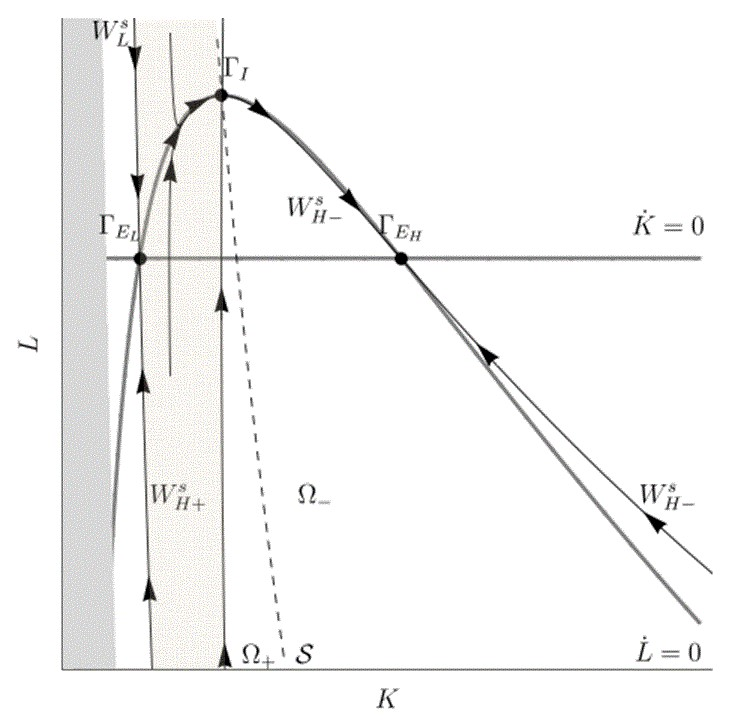
\includegraphics[scale=0.35]{phase_diagram}

\caption{Phase diagram for the endogenous tax rule model.}
\label{fig:phase_diagram.}

\end{figure}

	\subsection{Quotations}

Excerpts from others’ work should be used only when strictly necessary. Whenever used, it should be easy to identify their both presence in the text (using indentation and/or a different font) and their source.

For excerpts up to three lines, you can use the normal formatting of the body of the text e.g.: “as referred to by Rodrigues (2014), the final report is limited to a «maximum of 20 pages of text (…), including the table of contents.»”

Longer quotations should appear as follows:

\begin{displayquote}
{\small Recent research has also emphasized the role of imperfect competition in explaining a host of issues in international trade and finance (...). Thus, while there plainly are many other important distortions in the economy, there is good reason to believe that imperfect competition is one of the more important issues.}
\begin{flushright}
In: Obstfeld \& Rogoff (1996), p. 689.
\end{flushright}
\end{displayquote}

Unacknowledged use of another’s work is \textbf{plagiarism}. This not only violates the most basic rules of academic work, but as a form of falsification (or in some very specific cases, usurpation) it is also subject to disciplinary penalties imposed by the higher education institution. It is also a civil crime with penalties ranging from a fine to 3 years in prison (doubled in the case of repeat offences).

	\subsection{References}

Given the complexity of managing a bibliographical database linked to a text, especially on a large scale, such as in a MFW or doctoral thesis, use of specialist software (e.g. BibTeX, EndNote, ProCite, Reference Manager) is highly recommended from the beginning\footnote{I did not use software here, so that this template could be read by everyone.}. Reference databases such as EconLit or the Web of Knowledge export their listings into most formats used by these programmes, thereby facilitating the construction of a bibliography.

For formats to be used in-text and in the reference list, please read Costa (2017). Remember that there must be a one-to-one correspondence between the set of in-text citations (e.g. Costa, 2017 used above) and the list in the post-textual section References (e.g. Costa, L. (2017). \textit{Rules Governing the Presentation of Written Work at ISEG}. Mimeo ISEG.).


\begin{figure}[h]%Include figures.
\centering

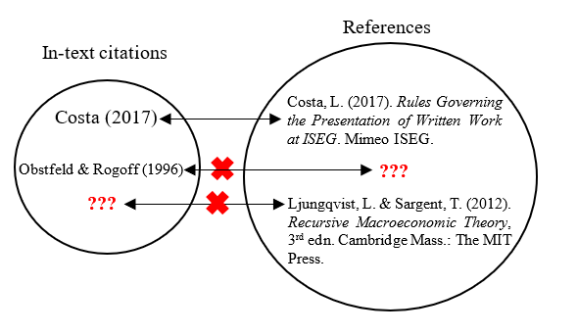
\includegraphics[scale=0.8]{citation_errors}

\caption{In-text citations and the reference list.}
\label{fig:citation_errors}

\end{figure}

Figure \ref{fig:citation_errors} above shows two examples of the wrong way of citing your bibliographic references:

\begin{itemize}
\item If you cite Obstfeld \& Rogoff (1996) in your text\footnote{I did it above.}, then you have to list it in the References section.
\item If you want to keep the book "Recursive Macroeconomic Theory" in your reference list, then you have to cite it in the text as "Ljungqvist \& Sargent (2012)".
\end{itemize}


\section{Conclusion}

This is the final section of the main text. The maximum length is 10 per cent of the textual part, i.e. 3.5 pages.

Here, you should present the results and (if applicable) your intentions for future research.

%  ==============    BIBLIOGRAPHY  ================

% NOTE: The use of a bibliographic manager is highly recommendable. One can import the references stored on a bibliographic manager, as examplified below (It is ommited for convenience).
%\addcontentsline{toc}{chapter}{Bibliography}
%\bibliographystyle{agsm}
%\bibliography{References} % <- insert you *.bib file here 

\clearpage
\begin{thebibliography}{9}

\item
Costa, L. (2017). \textit{Rules Governing the Presentation of Written Work at ISEG}. Mimeo ISEG.

\item
Obstfeld, M. \& Rogoff, K. (1996). \textit{Foundations of International Macroeconomics}. Cambridge Mass.: MIT Press.

\item
Rodrigues, C.F. (2014). \textit{Seminário da Licenciatura em Economia: Normas de elaboração do relatório final}. Mimeo ISEG.

\item
Romer, D. (2012). \textit{Advanced Macroeconomics}, 4th Ed. New York: McGraw-Hill.

\end{thebibliography}

%  ==============    APPENDIX: AFTER THIS POINT  ================

%\Appendices
\newpage
\begin{appendices}
\section{Title of the appendix A} \label{chap:appendixA}
\subsection{Section 1} \label{sec:A1}


\end{appendices}

\end{document}







